\subsubsection{Axes}

\begin{tabular}{|c|c|c|c|} \hline 
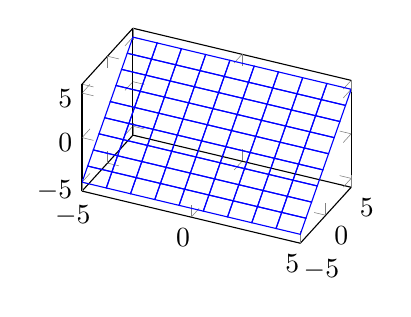
\begin{tikzpicture}
\begin{axis}[width=5cm,samples=10,mesh,no marks,plot box ratio=2 1 1]
\addplot3 {y};
\end{axis}
\end{tikzpicture}
&
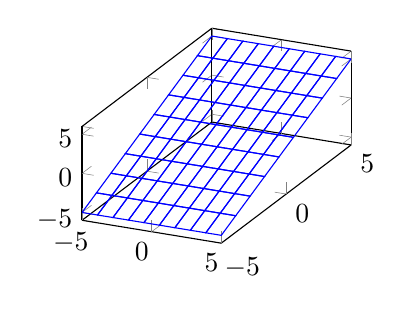
\begin{tikzpicture}
\begin{axis}[width=5cm,samples=10,mesh,no marks,plot box ratio=1 2 1]
\addplot3 {y};
\end{axis}
\end{tikzpicture}
&
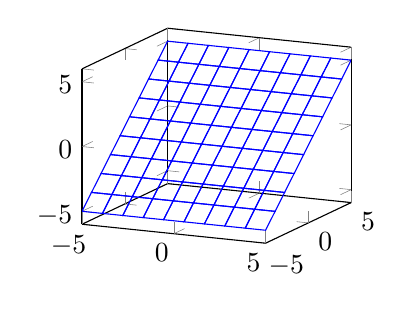
\begin{tikzpicture}
\begin{axis}[width=5cm,samples=10,mesh,no marks,plot box ratio=1 1 2]
\addplot3 {y};
\end{axis}
\end{tikzpicture}
 \\ \hline 
 plot box ratio=2 1 1 & plot box ratio=1 2 1 & plot box ratio=1 1 2
 \\ \hline   
 \end{tabular}

\bigskip
\begin{tabular}{|c|c|c|c|} \hline 
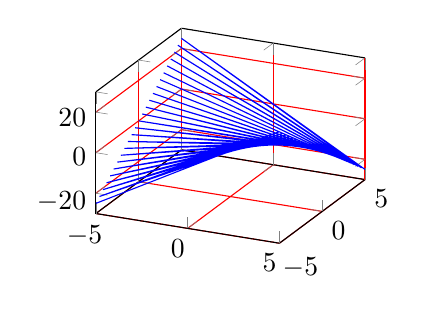
\begin{tikzpicture}
\begin{axis}[width=5cm,3d box=background,grid=major,grid style=red]
\addplot3 [blue] {-x*y};
\end{axis}
\end{tikzpicture}
&
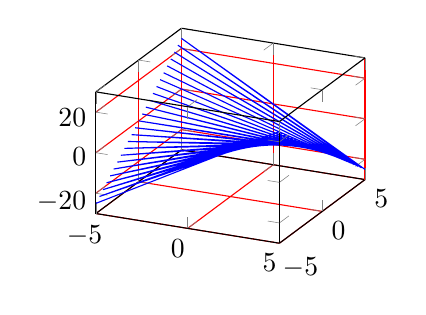
\begin{tikzpicture}
\begin{axis}[width=5cm,3d box=complete,grid=major,grid style=red]
\addplot3 [blue]  {-x*y};
\end{axis}
\end{tikzpicture}
&
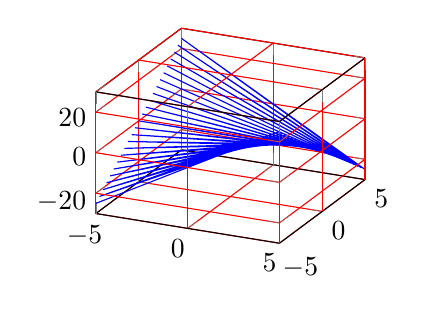
\begin{tikzpicture}
\begin{axis}[width=5cm,3d box=complete*,grid=major,grid style=red]
\addplot3  [blue] {-x*y};
\end{axis}
\end{tikzpicture}
 \\ \hline 
3d box=background (\dft) & 3d box=complete & 3d box=complete* 
 \\ \hline   
 \end{tabular}


\bigskip
\begin{tabular}{|c|c|c|c|} \hline  
 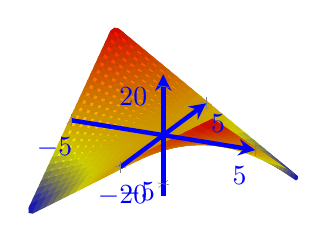
\begin{tikzpicture}
 \begin{axis}[width=5cm,axis lines=center,axis on top,ultra thick,blue]
 \addplot3[surf] {-x*y};
 \end{axis}
 \end{tikzpicture}
& 
  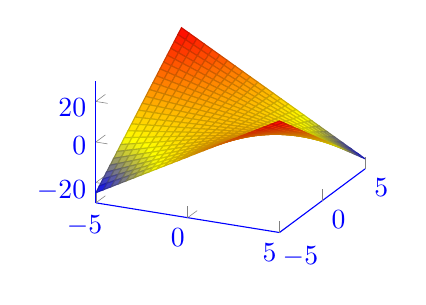
\begin{tikzpicture}
  \begin{axis}[width=5cm,axis lines*=left,blue]
  \addplot3[surf] {-x*y};
  \end{axis}
  \end{tikzpicture}
  &
 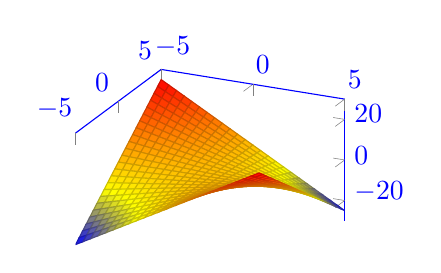
\begin{tikzpicture}
 \begin{axis}[width=5cm,axis lines*=right,blue]
\addplot3[surf] {-x*y};
\end{axis}
\end{tikzpicture}
\\ \hline 
axis lines=center,axis on top & axis lines*=left & axis lines*=right
\\ \hline 
  \end{tabular}


 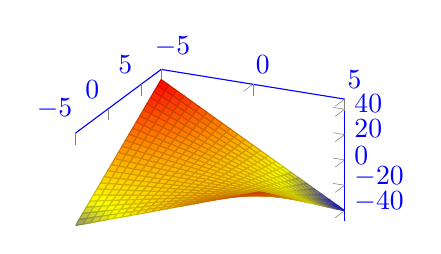
\begin{tikzpicture}
 \begin{axis}[width=5cm,axis lines*=right,blue,domain y=-5:(8)]
\addplot3[surf] {-x*y};
\end{axis}
\end{tikzpicture}
 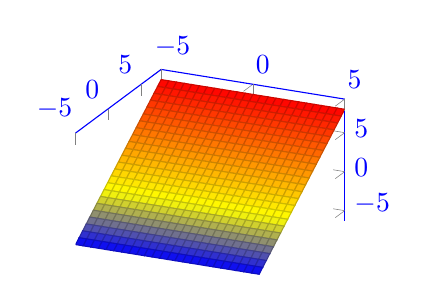
\begin{tikzpicture}
 \begin{axis}[width=5cm,axis lines*=right,blue,domain y=-5:(8)]
\addplot3[surf] {y};
\end{axis}
\end{tikzpicture}

 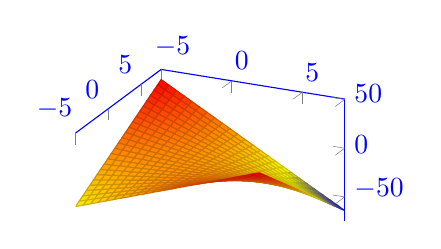
\begin{tikzpicture}
 \begin{axis}[width=5cm,axis lines*=right,blue,domain=-5:(8)]
\addplot3[surf] {-x*y};
\end{axis}
\end{tikzpicture}
 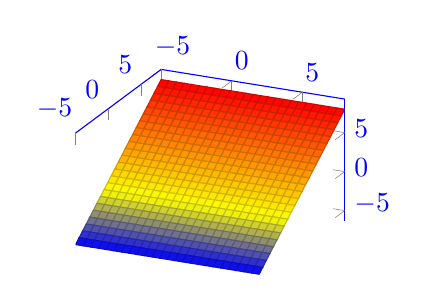
\begin{tikzpicture}
 \begin{axis}[width=5cm,axis lines*=right,blue,domain=-5:(8)]
\addplot3[surf] {y};
\end{axis}
\end{tikzpicture}

\SbSbSSCT{Tracé de la courbe}{Graph drawing}

\begin{tabular}{|c|c|c|c|} \hline 
\multicolumn{3}{|c|}{  \BS{addplot3}  [surf]  \AC{y};   }
\\ \hline
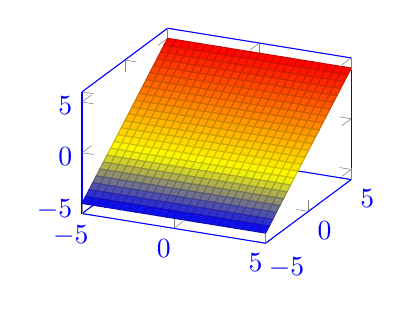
\begin{tikzpicture}
\begin{axis}[width=5cm,blue]
\addplot3 [surf] {y};
\end{axis}
\end{tikzpicture}
&
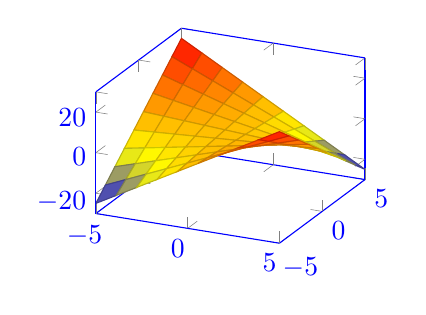
\begin{tikzpicture}
\begin{axis}[width=5cm,samples=10,blue]
\addplot3 [surf]  {-x*y};
\end{axis}
\end{tikzpicture}
&

\\ \hline 
\AC{y} & \AC{-x*y} &  gnuplot[id=sinxy]\AC{sin(x)*sin(y)};
\\ \hline 
\end{tabular}

\bigskip

\begin{tabular}{|c|c|c|c|} \hline 
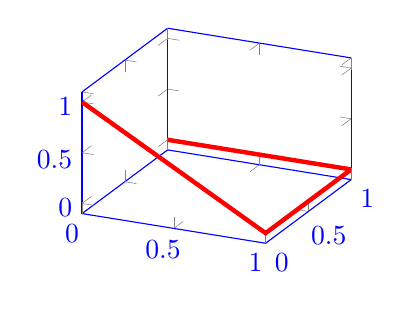
\begin{tikzpicture}
\begin{axis}[width=5cm,blue]
\addplot3[red,ultra thick] coordinates {(0,0,1) (1,0,0) (1,1,0) (0,1,0)};
\end{axis}
\end{tikzpicture}
&
\begin{tikzpicture}
\begin{axis}[width=5cm,blue]
\addplot3[red,ultra thick] file {table3.dat};
\end{axis}
\end{tikzpicture}
&
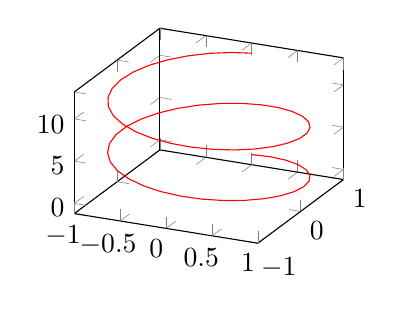
\begin{tikzpicture}
\begin{axis}[width=5cm,domain=0:720,samples=60,samples y=0]
\addplot3[red] ({sin(x)},{cos(x)},{x/60});
\end{axis}
\end{tikzpicture}
\\ \hline 
coordinates \AC{(0,0,1) (1,0,0) (1,1,0) (0,1,0)}; & file \AC{table3.dat}; & \AC{sin(x)},\AC{cos(x)},\AC{x/60});
\\ \hline 
\end{tabular}
\bigskip



\begin{tabular}{|p{1cm}  p{2cm} p{2cm} p{2cm} |} \hline
\multicolumn{4}{|c|}{\TFRGB{Contenu du fichier}{content of the file} table3.dat}
\\ \hline
& 0 & 0 & 0 \\
& 0 & 0.5 & 0 \\
& 0 & 1 & 1 \\
& 1 & 1 & 5  \\
& 1 & 0.5&  0 \\
& 1 & 0 &  0 \\

\hline
\end{tabular}


\subsubsection{Aspect}

\begin{tabular}{|c|c|c|c|} \hline 
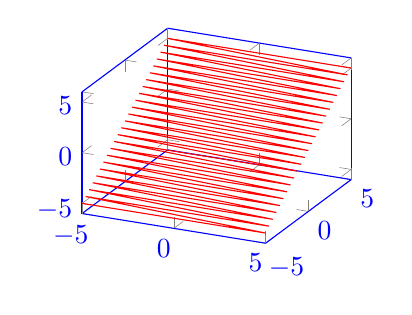
\begin{tikzpicture}
\begin{axis}[width=5cm,blue]
\addplot3 [red] {y};
\end{axis}
\end{tikzpicture}
&
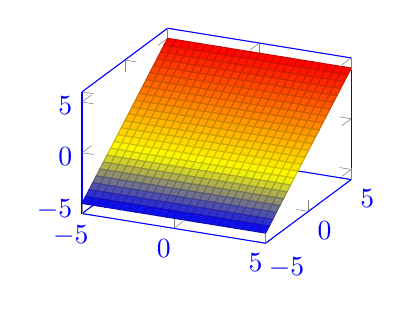
\begin{tikzpicture}
\begin{axis}[width=5cm,blue]
\addplot3 [surf] {y};
\end{axis}
\end{tikzpicture}
&
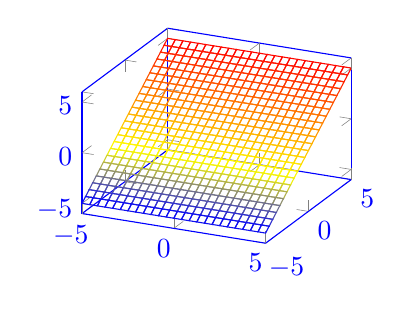
\begin{tikzpicture}
\begin{axis}[width=5cm,blue]
\addplot3 [mesh] {y}; 
\end{axis}
\end{tikzpicture}
 \\ \hline 
[red] & [\RDD{surf}] & [\RDD{mesh}]
\\ \hline 
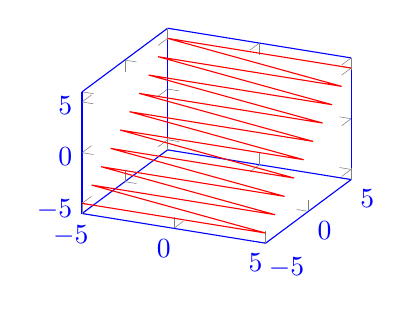
\begin{tikzpicture} 
\begin{axis}[width=5cm,blue]
\addplot3 [red,samples=10]{y};
\end{axis}
\end{tikzpicture}
&
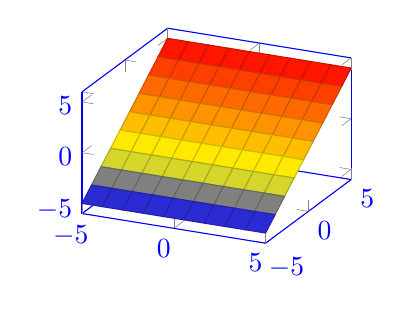
\begin{tikzpicture}
\begin{axis}[width=5cm,blue]
\addplot3 [surf,samples=10] {y};
\end{axis}
\end{tikzpicture}
&
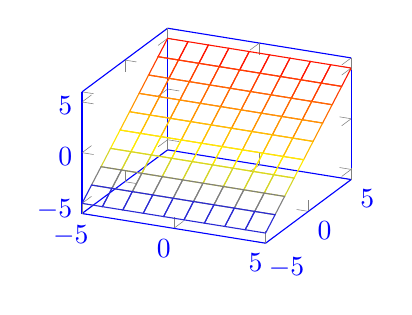
\begin{tikzpicture}
\begin{axis}[width=5cm,blue]
\addplot3 [mesh,samples=10] {y};
\end{axis}
\end{tikzpicture}
 \\ \hline 
[red,samples=10] & [surf,samples=10] & [mesh,samples=10]
\\ \hline  
\end{tabular}
\bigskip

\begin{tabular}{|c|c|c|c|} \hline 
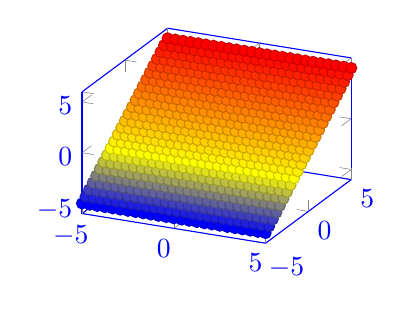
\begin{tikzpicture}
\begin{axis}[width=5cm,blue]
\addplot3 [scatter] {y};
\end{axis}
\end{tikzpicture}
&
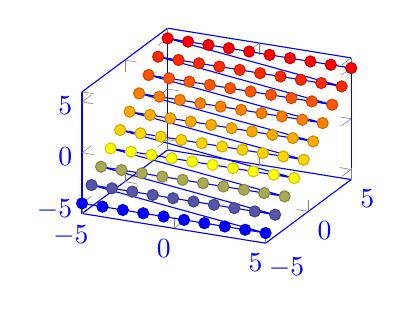
\begin{tikzpicture}
\begin{axis}[width=5cm,blue]
\addplot3 [scatter,samples=10] {y};
\end{axis}
\end{tikzpicture}
&
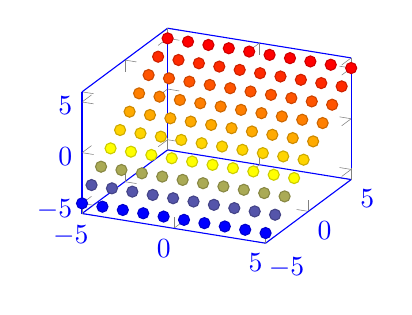
\begin{tikzpicture}
\begin{axis}[width=5cm,blue]
\addplot3 [scatter,samples=10,only marks] {y};
\end{axis}
\end{tikzpicture}
\\ \hline  
[scatter] & [scatter,samples=10] & [scatter,samples=10,only marks]
\\ \hline  
\end{tabular}

\bigskip 

\begin{tabular}{|c|c|c|c|} \hline 
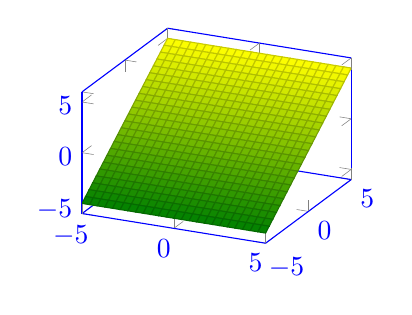
\begin{tikzpicture}
\begin{axis}[width=5cm,blue]
\addplot3 [surf,colormap/greenyellow] {y};
\end{axis}
\end{tikzpicture}
&
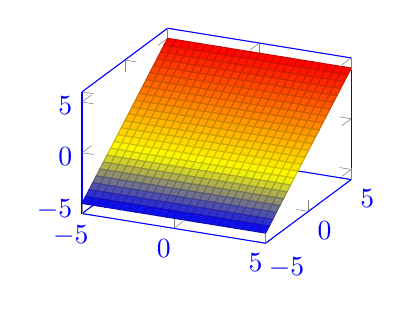
\begin{tikzpicture}
\begin{axis}[width=5cm,blue]
\addplot3 [surf,colormap/hot] {y};
\end{axis}
\end{tikzpicture}
&
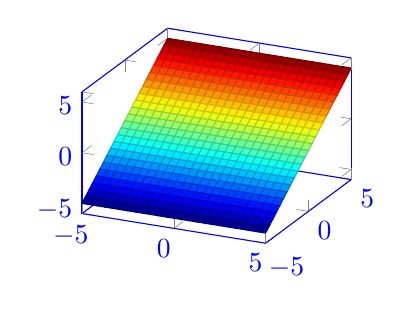
\begin{tikzpicture}
\begin{axis}[width=5cm,blue]
\addplot3 [surf,colormap/jet] {y};
\end{axis}
\end{tikzpicture}
\\ \hline 
[surf,\RDD{colormap/greenyellow}] & [surf,\RDD{colormap/hot}] & [surf,\RDD{colormap/jet}]
\\ \hline 
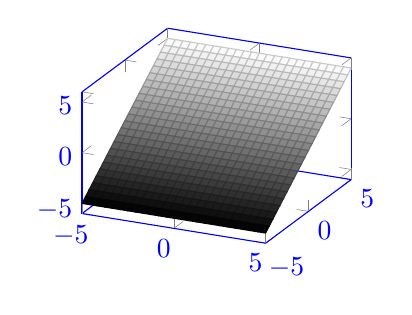
\begin{tikzpicture}
\begin{axis}[width=5cm,blue]
\addplot3 [surf,colormap/blackwhite] {y};
\end{axis}
\end{tikzpicture}
&
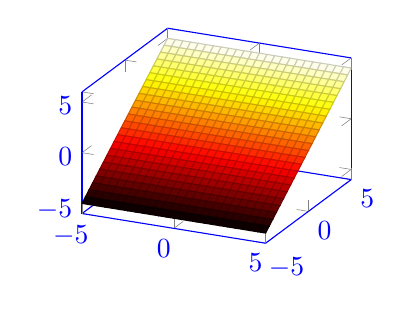
\begin{tikzpicture}
\begin{axis}[width=5cm,blue]
\addplot3 [surf,colormap/hot2] {y};
\end{axis}
\end{tikzpicture}
&
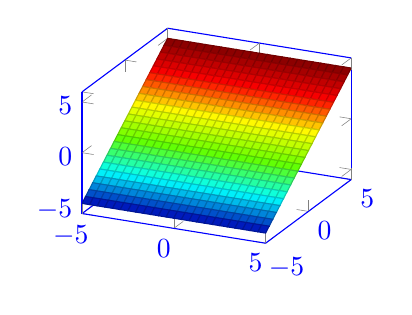
\begin{tikzpicture}
\begin{axis}[width=5cm,blue]
\addplot3 [surf,colormap/bluered] {y};
\end{axis}
\end{tikzpicture}
\\ \hline
[surf,\RDD{colormap/blackwhite}] & [surf,\RDD{colormap/hot2}] & [surf,\RDD{colormap/bluered}]
\\ \hline 
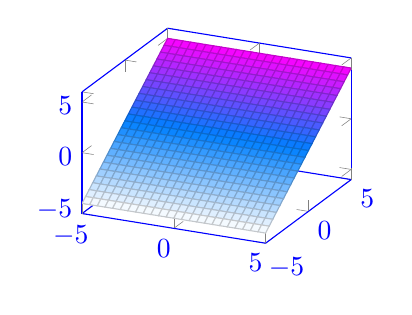
\begin{tikzpicture}
\begin{axis}[width=5cm,blue]
\addplot3 [surf,colormap/cool] {y};
\end{axis}
\end{tikzpicture}
&
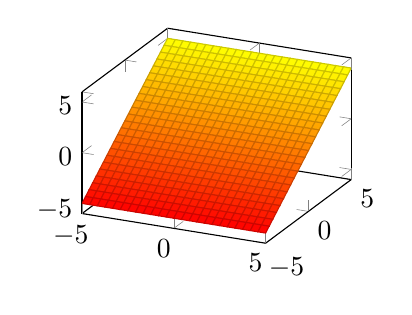
\begin{tikzpicture}
\begin{axis}[width=5cm]
\addplot3 [surf,colormap/redyellow] {y};
\end{axis}
\end{tikzpicture}
&
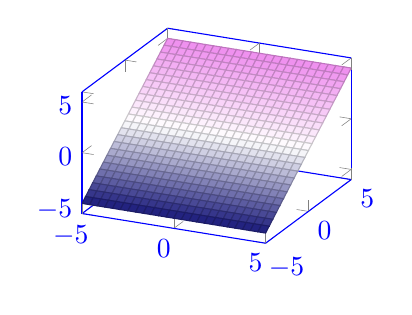
\begin{tikzpicture}
\begin{axis}[width=5cm,blue]
\addplot3 [surf,colormap/violet] {y};
\end{axis}
\end{tikzpicture}
\\ \hline 
[surf,\RDD{colormap/cool}] & [surf,\RDD{colormap/redyellow}] & [surf,\RDD{colormap/violet}]
\\ \hline 
\end{tabular}



\bigskip 

\begin{tabular}{|c|c|c|c|} \hline 
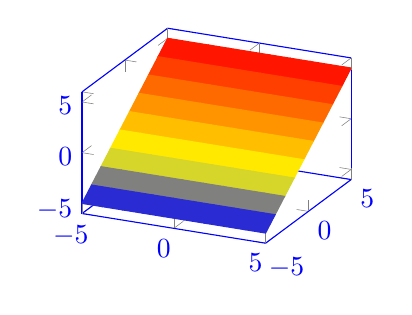
\begin{tikzpicture}
\begin{axis}[width=5cm,blue]
\addplot3 [surf,shader=flat,samples=10] {y};
\end{axis}
\end{tikzpicture}
&
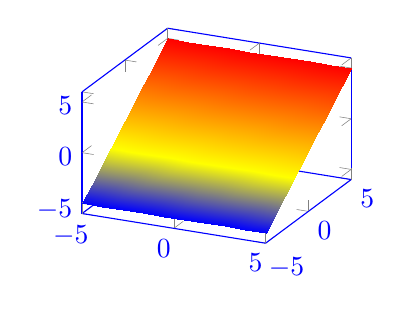
\begin{tikzpicture}
\begin{axis}[width=5cm,blue]
\addplot3 [surf,shader=interp,samples=10] {y};
\end{axis}
\end{tikzpicture}
&
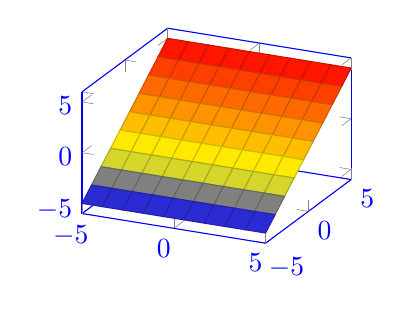
\begin{tikzpicture}
\begin{axis}[width=5cm,blue]
\addplot3 [surf,shader=faceted,samples=10] {y};
\end{axis}
\end{tikzpicture}
\\ \hline
\RDD{shader}=flat & \RDD{shader}=interp & \RDD{shader}=faceted
 \\ \hline 
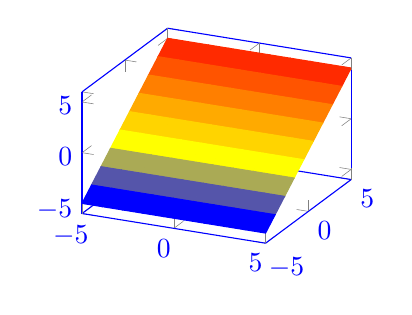
\begin{tikzpicture}
\begin{axis}[width=5cm,blue]
\addplot3 [surf,shader=flat corner,samples=10] {y};
\end{axis}
\end{tikzpicture}
&
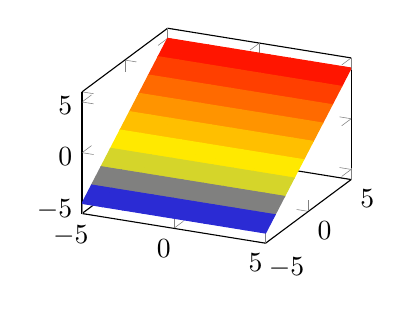
\begin{tikzpicture}
\begin{axis}[width=5cm]
\addplot3 [surf,shader=flat mean,samples=10] {y};
\end{axis}
\end{tikzpicture}
&
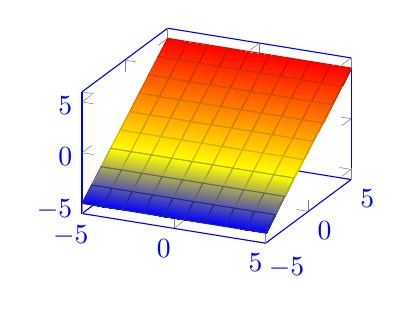
\begin{tikzpicture}
\begin{axis}[width=5cm,blue]
\addplot3 [surf,shader=faceted interp,samples=10] {y};
\end{axis}
\end{tikzpicture}
 \\ \hline 
\RDD{shader}=flat corner &  \RDD{shader}=flat mean & \RDD{shader}=faceted interp 
 \\ \hline   
 \end{tabular}


%A Voir-------------------------------------------------



%\begin{tikzpicture}
%\begin{axis}[width=5cm]
%\addplot3[mesh,domain=0:360] {sin(x)*sin(y)};
%\end{axis}
%\end{tikzpicture}
%\begin{tikzpicture}
%\begin{axis}[width=5cm]
%\addplot3[surf,fill=white,domain=0:360] {sin(x)*sin(y)};
%\end{axis}
%\end{tikzpicture}

%\begin{tikzpicture}
%\begin{axis}[width=5cm,axis background/.style={fill=red!10}]
%\addplot3 [blue] {y};
%\end{axis}
%\end{tikzpicture}


%\begin{tikzpicture}
%\begin{axis}[
%axis lines=center,
%axis on top,
%xlabel={$x$}, ylabel={$y$}, zlabel={$z$},
%domain=0:1,
%y domain=0:2*pi,
%xmin=-1.5, xmax=1.5,
%ymin=-1.5, ymax=1.5, zmin=0.0,
%mesh/interior colormap=
%{blueblack}{color=(black) color=(blue)},
%colormap/blackwhite,
%samples=10,
%samples y=40,
%z buffer=sort,
%]
%\addplot3[surf]
%({x*cos(deg(y))},{x*sin(deg(y))},{x});
%\end{axis}
%\end{tikzpicture}
